\section{Introducción}

La comunicación es uno de los ejes fundamentales de la humanidad, a lo largo de la historia han aparecido diferentes medios para poder satisfacer esta necesidad, sin embargo el concepto nunca se había formalizado. En 1948, el matemático e ingeniero Claude E. Shannon propone una definición formal de que es la comunicación desde una punto de vista matemático, dando origen a la \textit{Teoría de la Información}. En este trabajo analizaremos como aplica dicha teoría a un medio de comunicación real, particularmente uno que sea altamente utilizado y tenga una alta densidad de usuarios.

\section{Desarrollo}

\subsection{Informacion y Entropia}

Como vimos en la introduccion, en 1948 el matematico Claude E. Shannon define formalmente que es la \textit{Información} en su publicación \textit{A Mathematical Theory of Communication}, junto con esta defincion tambien introduce el concepto de \textit{Entropia} en la comunicación. Primero definimos quienes son los participes en la comunicación:

\begin{itemize}
	\item Fuente de Informacion
	\item Emisor
	\item Receptor
	\item Destino de Informacion
	\item Ruido
	\item Canal
\end{itemize}

Los mismos se encuentran conectados de la siguiente forma:

\begin{figure}[ht]
\begin{center}
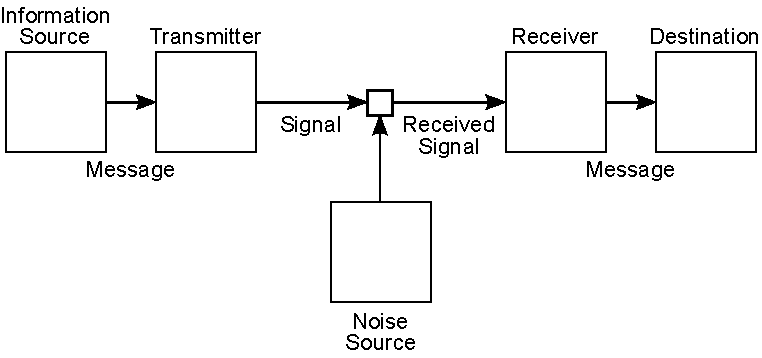
\includegraphics[width=0.6\columnwidth]{graficos/Shannon.pdf}
\caption{Diagrama de comunicación}
\end{center}
\end{figure}

Para poder establecer una comunicación punto a punto, es necesario que el emisor y el receptor "`hablen"' un lenguaje en común. Para poder satisfacer esto, se define un conjunto de símbolos $S = \{ s_1, ..., s_n \}$, con una probabilidad $p(s_i)$ con $1 \leq i \leq n$ asociada a cada uno de ellos, este conjunto representa la totalidad de símbolos que pueden ser transmitidos por el canal. Una vez definido el conjunto, la información que se obtiene por símbolo es simplemente $I(s_i) = log(\frac{1}{p(s_i)})$. Se elige el logaritmo como función por cumplir con varias condiciones idóneas para calcular la informacion, de las mas interesantes tenemos que:

\begin{itemize}
	\item Si $s \in S$, entonces $I(s) \geq 0$. Esto vale ya que la inversa de la probabilidad es siempre mayor o igual a 1
	\item Si $p(s_i) = 1$ para algun $i$, entonces $I(s_i) = 0$, ya que un evento que ocurre siempre no aporta información significativa
	\item $I(s_i, s_j) \leq I(s_i) + I(s_j)$, la igualdad vale unicamente si los símbolos son independientes
\end{itemize}

Como podemos apreciar, la función logaritmo cumple con todos estos puntos.

En nuestro trabajo analizaremos principalmente la entropia, esta se define como $H(S) = \sum\limits_{i=1}^n p(s_i)I(s_i)$. Esta medida representa la media de información obtenida por símbolo en la comunicación, y se encuentra íntimamente relacionada con las probabilidades de cada símbolo, particularmente mientras menos aleatoria sea una red, menor es la entropia. También aplica el mismo razonamiento a la inversa, es decir, mientras mas cerca de la equiprobabilidad estén los símbolos, la entropia aumentara, maximizándose cuando los símbolos sean equiprobables.

%Antes de proceder a describir la metodologia para los experimentos, consideramos pertinente dar una interpretacion de la entropia. Podemos ver que esta medida esta relacionada con la probabilidad de cada simbolo, mientras menos informacion tengamos acerca de los símbolos, es natural asumir que estos se encuentran cerca de la equiprobabilidad. Sin embargo, a medida que tengamos mas conocimiento acerca de las posibilidades de aparición de cada símbolo, la entropia del canal va a bajar, ya que en los simbolos mas comunes no nos van aportar de informacion significativa. Esto lo podemos apreciar comparando los lenguajes basados en alfabeto reducido y los basados en pictogramas, si tomamos el caso del español que esta basado en el alfabeto latino, podemos ver que ciertas letras aparecen con mucho mas frecuencia que otras con lo cual la entropia tiende a ser menor, mientras que en el caso de lenguajes como el chino, al ser tan densos (el chino básico tiene hasta 50000 pictogramas) estimar las probabilidades se vuelve una tarea complicada, llevando a que la entropia sea mayor.

\subsection{Canal elegido}

Para poder tener suficientes datos para hacer un análisis interesante, seria prudente tomar un medio que sea ampliamente usado. Por ello, elegimos utilizar una red del tipo Wi-Fi, los puntos a destacar de la red son:

\begin{itemize}
	\item En la aplicaciones habituales, estas redes se caracterizan por tener un \textit{nodo} central, el cual se encarga de regular el trafico en la red
	\item En las redes publicas, los nodos que no son el central no se suelen comunicar entre ellos, estos principalmente se conectan con servidores en Internet
\end{itemize}

\subsection{Paquetes de red}

En la redes la información en el canal se transmite en paquetes, estos paquetes tienen varios campos, particularmente nos interesan analizar los paquetes de capa 2 y capa 3. De los paquetes \textit{Ethernet} de capa 2, nos interesa:

\begin{itemize}
	\item Dirección MAC de origen
	\item Dirección MAC de destino
	\item Protocolo del payload, este depende del paquete de capa 3 que se esta transportando, puede ser IPv4, IPv6, ARP, etc.
\end{itemize}

Por otro lado, de los paquetes de capa 3 nos interesan solamente los ARP. De este tipo de paquetes nos interesan los campos:

\begin{itemize}
	\item Tipo de operación
	\item Dirección MAC del emisor
	\item Dirección IP del emisor
	\item Dirección MAC del destinatario
	\item Dirección IP del destinatario
\end{itemize}

El fin de los paquetes ARP, es vincular la capa 2 con la capa 3, relacionando las direcciones IP con direcciones MAC fisicas. Para hacer esto el protocolo ARP cuenta con dos operaciones, estas pueden ser \textit{who-has} o \textit{is-at}.

Las operaciones \textit{who-has} sirven para identificar a que dirección MAC física corresponda una dirección IP de la red, estos paquetes suelen ser de tipo \textit{broadcast}.

En respuesta a los \textit{who-has}, tenemos las operaciones \textit{is-at}. Una vez que un nodo recibe un paquete de tipo \textit{who-has}, este revisa si la dirección IP del mismo coincide con la suya, en el caso de que lo sea este enviá un paquete al nodo que genero el \textit{who-has} para notificarle su dirección MAC física.

Para no tener que enviar paquetes ARP por cada paquete IP que se desea enviar, el emisor del \textit{who-has} al recibir el \textit{is-at}, guarda el resultado en una tabla para poder enviar futuros paquetes al mismo destino inmediatamente.

\section{Metodología}

En el trabajo se pide que analicemos dos fuentes de información, estas son $S$ y $S_1$, y tienen la siguiente forma:

\begin{itemize}
	\item $S$: Comprende a todos los paquetes \textit{Ethernet} que circulan por el canal, se los diferencia por el \textit{protocolo} del payload.
	\item $S_1$: Se limita a los paquetes \textit{Ethernet} de tipo ARP.
\end{itemize}

\pagebreak

Para $S_1$ ademas se pide establecer un criterio de diferenciación, para esto tomamos la conjunción de las direcciones IP fuente y destino de los paquetes ARP de tipo \textit{who-has}. Elegimos estos paquetes ya que los \textit{is-at} se dan unicamente en respuesta a algún \textit{who-has} anterior, con lo cual estaríamos duplicando ciertos paquetes.

Las redes elegidas para \textit{sniffear} fueron las siguientes:

\begin{itemize}
	\item FibertelZone, en shopping Plaza Oeste Moron (60 min. de captura)
	\item Laboratorios-DC (30 min. de captura)
	\item Red hogareña (30 min. de captura)
\end{itemize}

Por ultimo, es pertinente definir que consideramos como símbolo distinguido. Siguiendo la definición de información, consideramos como símbolo distinguido aquel que provee la menor cantidad de información, si bien podríamos aplicar el mismo criterio a la inversa (es decir, considerar distinguido al nodo que mas información provea), nos interesa analizar al símbolo de menor información por las siguientes razones:

\begin{itemize}
	\item $S$: En este caso los nodos que mas apariciones tengan, van a ser los protocolos que dominen el trafico de la red. Debido a que el objetivo principal de las redes publicas Wi-Fi es acceder a Internet, nuestra teoría es que los paquetes IPv4 van a ser los que mas apariciones tengan, y a su vez los que menos información provean como símbolo (si bien IPv6 sirve para acceder a Internet, no se usa en la misma medida que IPv4)
	\item $S_1$: Aquí es mas interesante estudiar los paquetes que menos información provean, ya que tenemos la teoría de que en una red Wi-Fi convencional, el nodo que corresponde al enrutador va a ser el que mas aparezca de los paquetes ARP, ya que la mayoría del trafico pasa a través de el. Con lo cual dicho nodo no solamente seria el que mas aparezca en la red, sino que ademas la información que el mismo provee como símbolo sera mucho menor que la del resto de los nodos
\end{itemize}

%Inicialmente la idea era capturar paquetes en una mayor cantidad de redes, sin embargo, nos topamos con que en diferentes redes publicas el trafico no era suficientemente alto, con lo cual la captura de paquetes no era significativa ni suficiente como para hacer un analisis mas exhaustivo. Consideramos que esto se debe en parte al aumento en el uso de Smartphones con redes moviles, junto con la mala fama que tienen las redes Wi-Fi publicas.

\section{Resultados}

\subsection{Protocolos}

Vamos a ver primero la cantidad de paquetes en las redes, y la informacion que los mismos proveyeron como simbolos:

%\begin{figure}[H]
%\begin{center}
%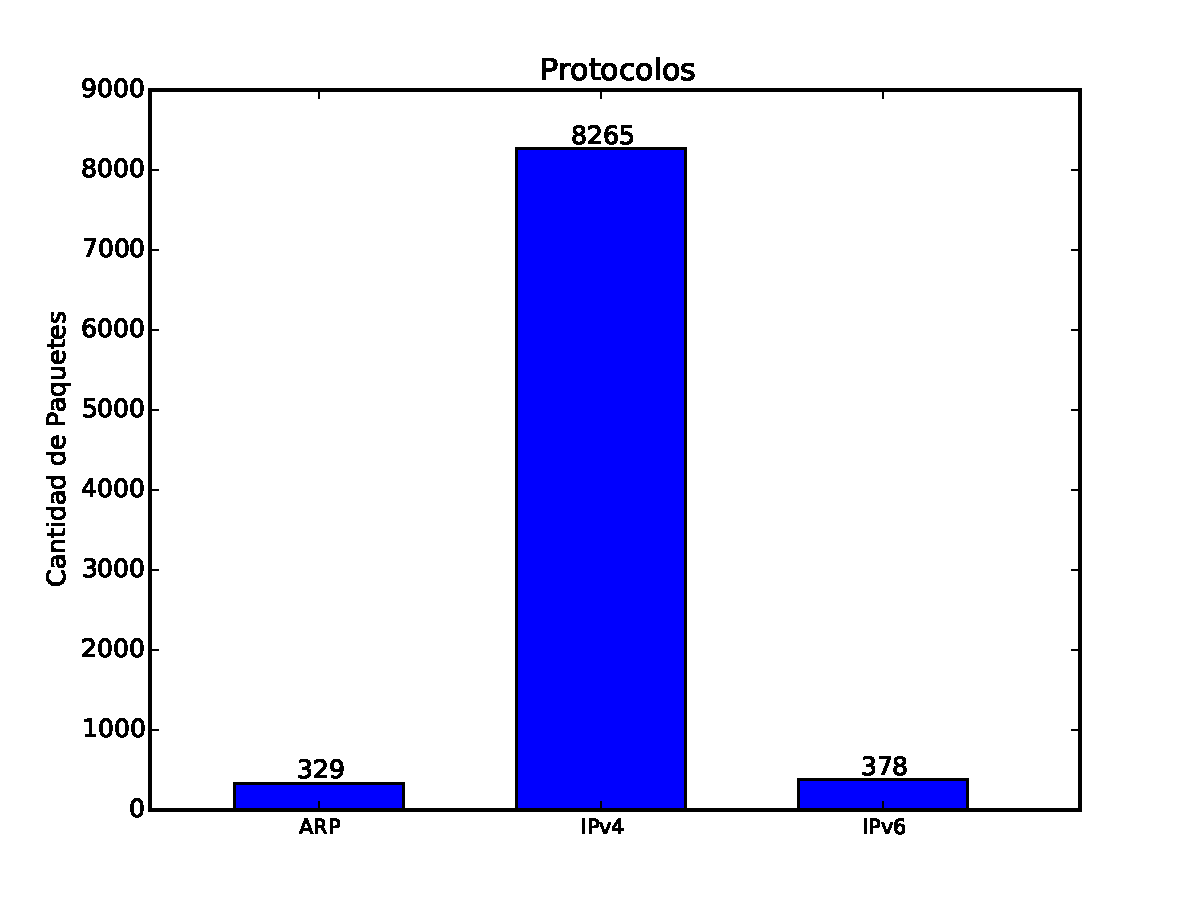
\includegraphics[width=0.8\columnwidth]{graficos/plaza_s1.pdf}
%\caption{Red Plaza Oeste}
%\end{center}
%\end{figure}

\begin{table}[H]
\centering
\caption{Red Plaza Oeste}
\label{my-label}
\begin{tabular}{@{}llll@{}}
\toprule
Tipo de paquete & Apariciones & Informacion & Apariciones / Total \\ \midrule
ARP             & 329         & 3.305       & 0.037               \\
IPv4            & 8265        & 0.082       & 0.921               \\
IPv6            & 378         & 3.166       & 0.042               \\ \bottomrule
\end{tabular}
\end{table}

%\begin{figure}[H]
%\begin{center}
%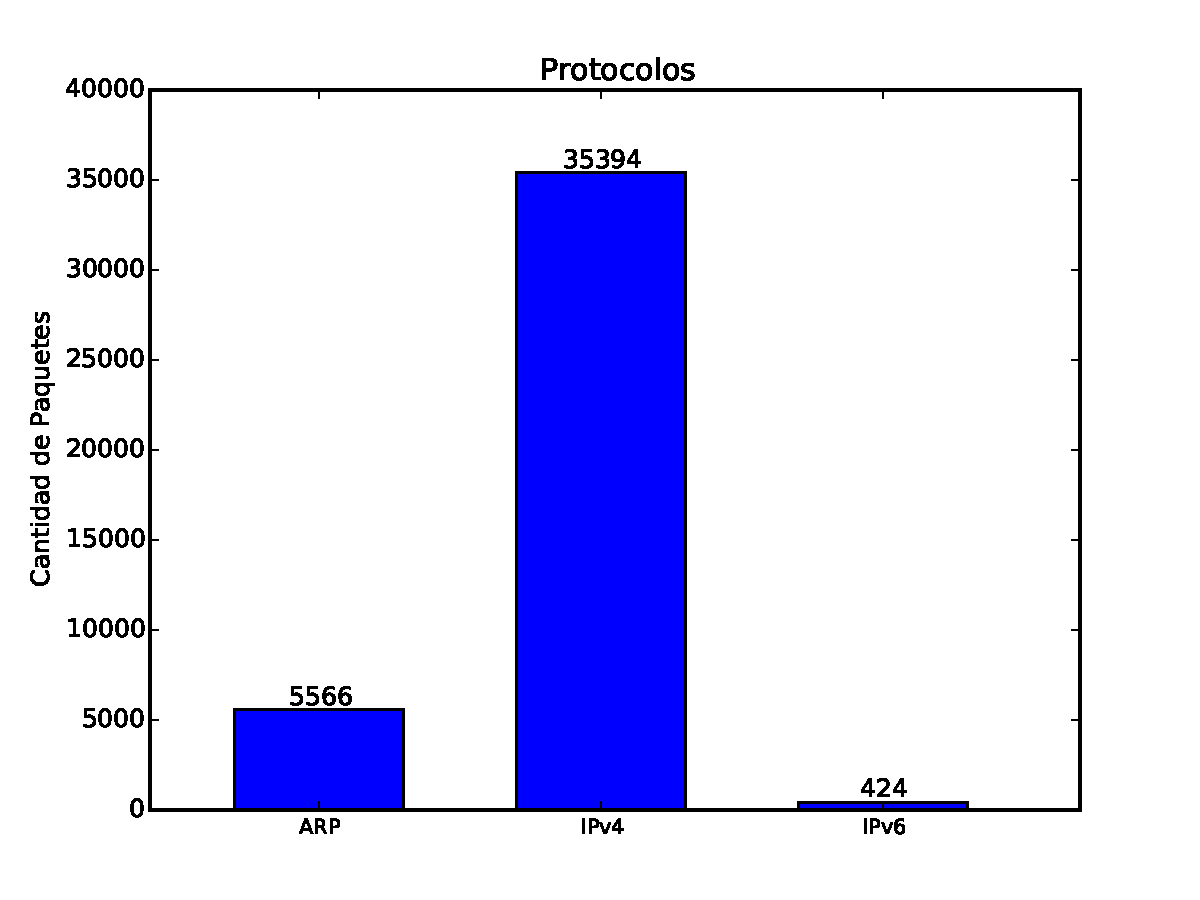
\includegraphics[width=0.8\columnwidth]{graficos/dc_s1.pdf}
%\caption{Red Laboratorios DC}
%\end{center}
%\end{figure}

\begin{table}[H]
\centering
\caption{Red Laboratorios DC}
\label{my-label}
\begin{tabular}{@{}llll@{}}
\toprule
Tipo de paquete & Apariciones & Informacion & Apariciones / Total \\ \midrule
ARP             & 5566        & 2.006       & 0.134               \\
IPv4            & 35394       & 0.156       & 0.855               \\
IPv6            & 424         & 4.580       & 0.011               \\ \bottomrule
\end{tabular}
\end{table}

%\begin{figure}[H]
%\begin{center}
%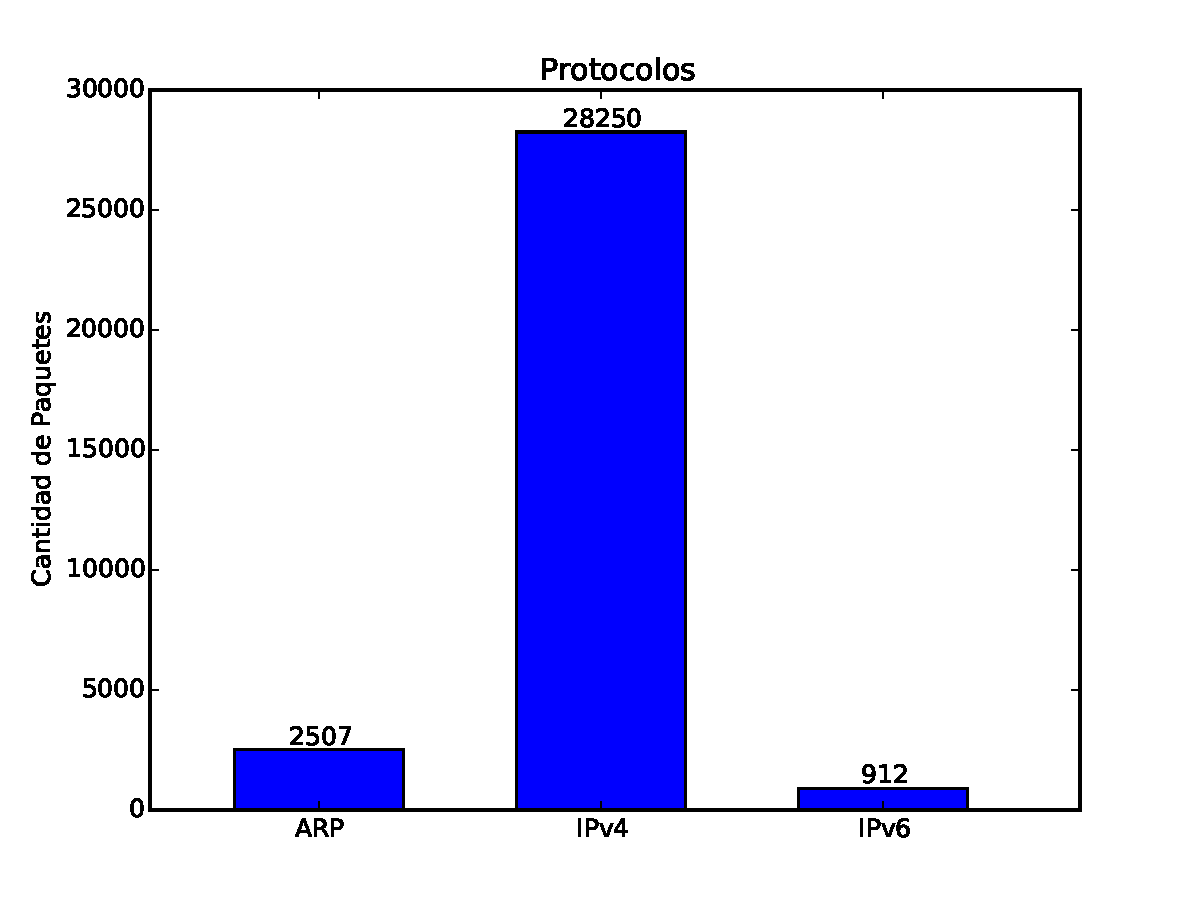
\includegraphics[width=0.8\columnwidth]{graficos/hogar_s1.pdf}
%\caption{Red hogareña}
%\end{center}
%\end{figure}

\begin{table}[H]
\centering
\caption{Red hogareña}
\label{my-label}
\begin{tabular}{@{}llll@{}}
\toprule
Tipo de paquete & Apariciones & Informacion & Apariciones / Total \\ \midrule
ARP             & 2507        & 2.536       & 0.079               \\
IPv4            & 28250       & 0.114       & 0.892               \\
IPv6            & 912         & 3.547       & 0.029               \\ \bottomrule
\end{tabular}
\end{table}

%Como podemos apreciar, los paquetes IPv4 dominan el trafico de la red. A continuación vamos a ver la información por símbolo junto con la entropia:
%
%\begin{figure}[H]
%\begin{center}
%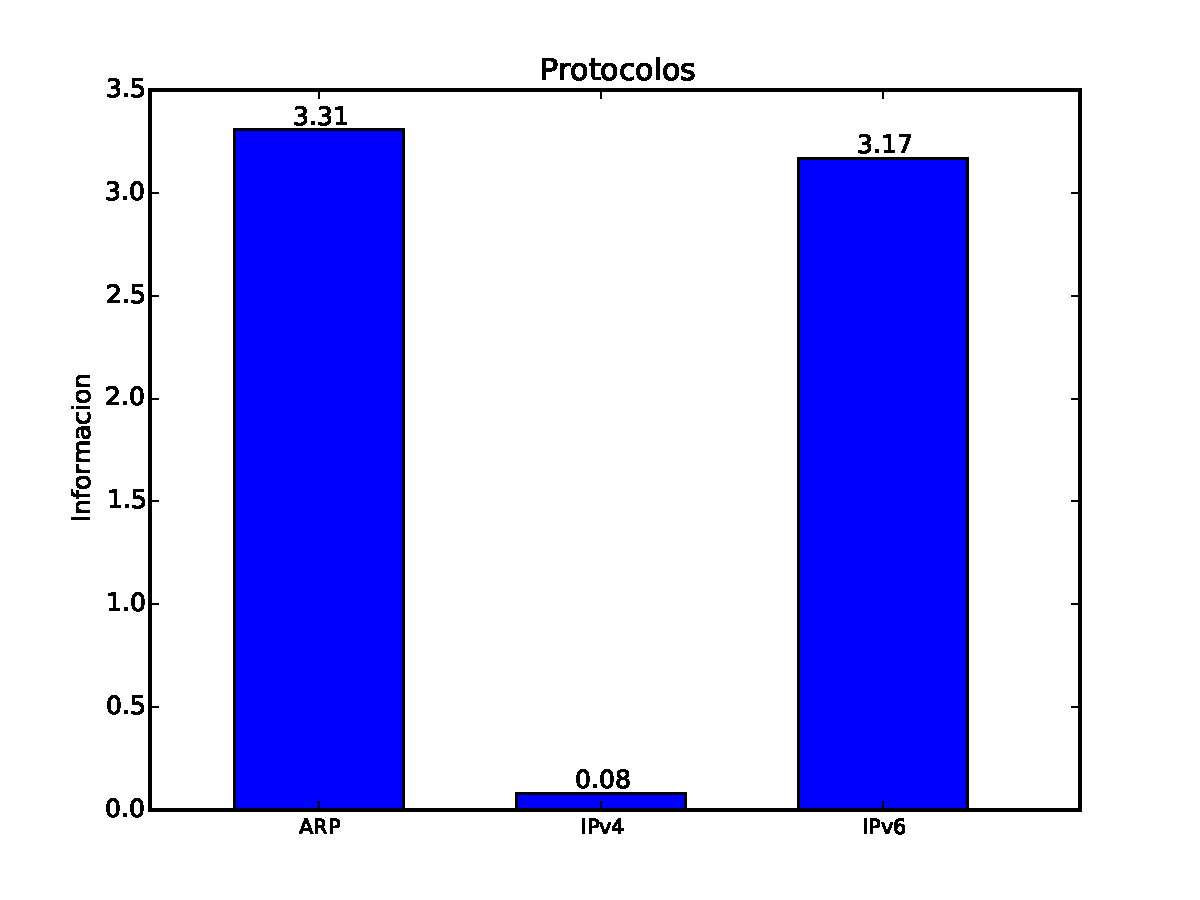
\includegraphics[width=0.7\columnwidth]{graficos/plaza_inf_s1.pdf}
%\caption{Red Plaza Oeste}
%\end{center}
%\end{figure}
%
%\begin{figure}[H]
%\begin{center}
%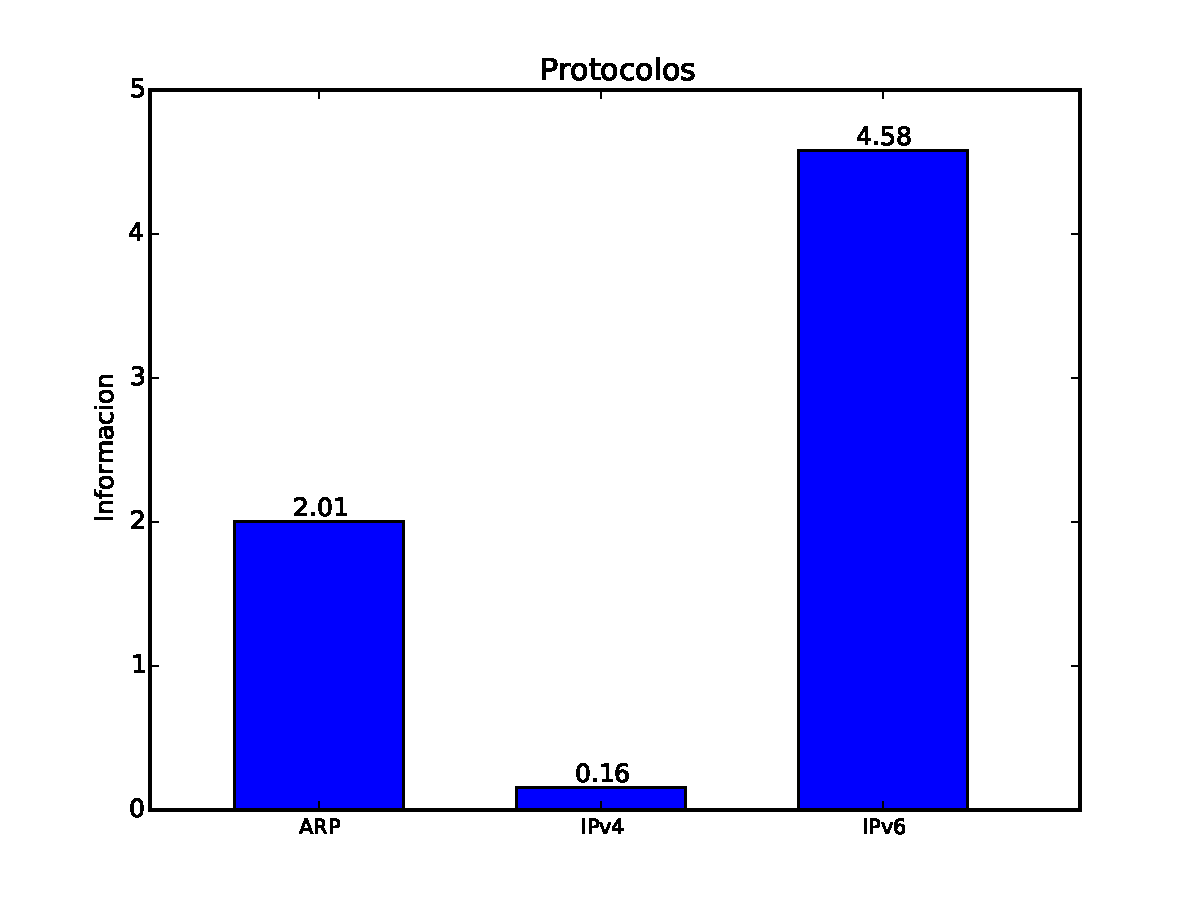
\includegraphics[width=0.7\columnwidth]{graficos/dc_inf_s1.pdf}
%\caption{Red Laboratorios DC}
%\end{center}
%\end{figure}
%
%\begin{figure}[H]
%\begin{center}
%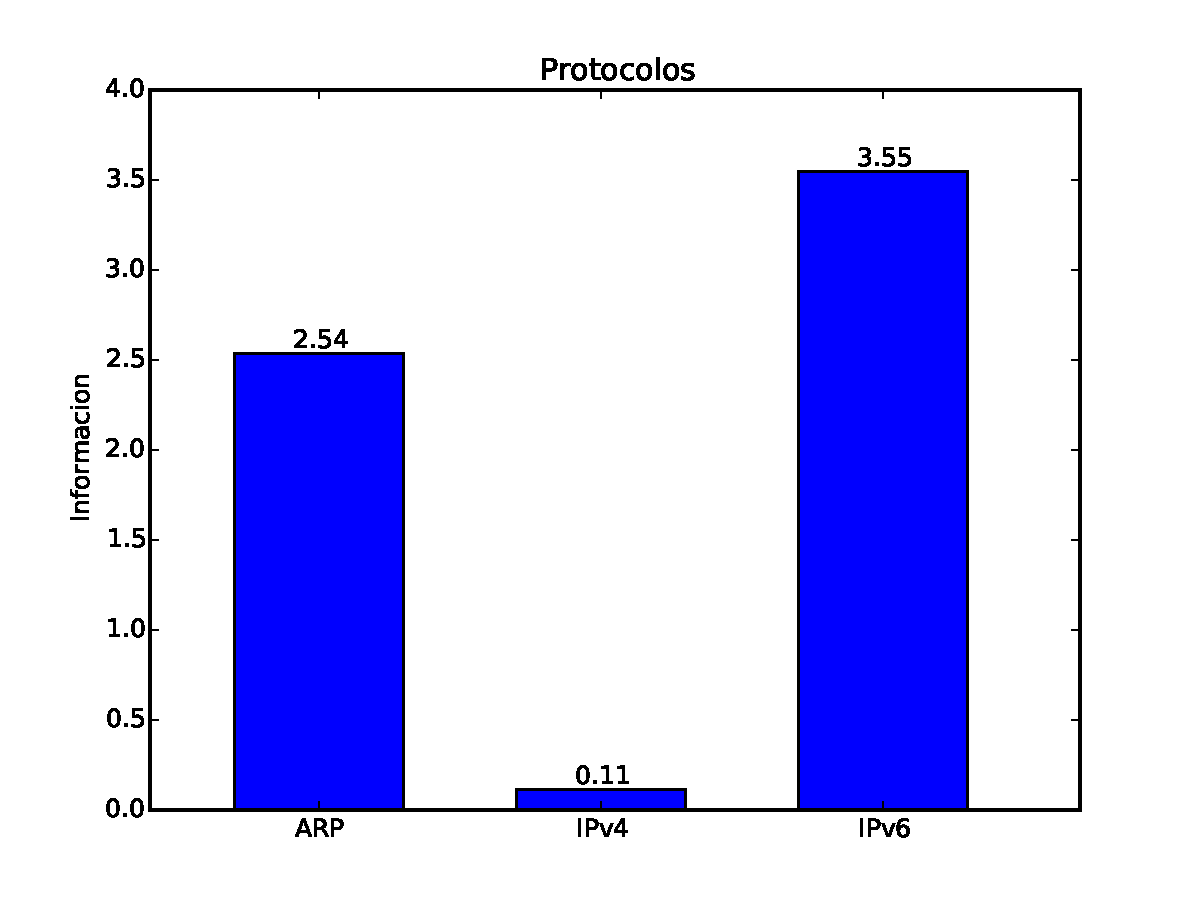
\includegraphics[width=0.8\columnwidth]{graficos/hogar_inf_s1.pdf}
%\caption{Red hogareña}
%\end{center}
%\end{figure}

\pagebreak

La entropia en las redes fue:

\begin{table}[H]
\centering
\caption{Entropia}
\label{my-label}
\begin{tabular}{ll}
\hline
Red         & Entropia \\ \hline
Plaza Oeste & 0.3303   \\
Laboratorios DC    & 0.4505   \\ 
Hogareña & 0.4048   \\  \hline
\end{tabular}
\end{table}

Debido a que la cantidad de símbolos es pequeña, decidimos poner en la tabla a todo el conjunto de símbolos de la fuente $S$.

Como podemos ver, la entropia de la red es bastante baja en ambos, esto se debe a la gran cantidad de paquetes IPv4 en ambos canales. Otro punto interesante es que en la red unicamente circulan paquetes de tipo ARP, IPv4 o IPv6, si bien esto es esperable en la red del Plaza Oeste y la red hogareña, nos sorprendió que ocurra también en la red Laboratorios DC, inicialmente creíamos que podía haber algún protocolo en la red que se use de manera casi exclusiva en algún software de índole académica. Sin embargo, el objetivo principal de las redes publicas es proveer de acceso a Internet a los usuarios de la misma, con lo cual el hecho de que solamente se encuentren este tipo de paquetes no es nada fuera de lo normal.

Nuestras predicciones indicaban que la mayoría de los paquetes iban a ser de tipo IPv4 por un margen bastante significativo, esto se corresponde con que la probabilidad de dicho paquete iba a ser mucho mas alta que el resto, con lo cual la información de dichos paquetes iba a ser considerablemente menor. Como la diferencia es tan amplia, por un margen muy significativo, siguiendo el criterio definido anteriormente, consideramos al protocolo IPv4 como símbolo distinguido.

\pagebreak

\subsection{Paquetes ARP}

Como vimos en el desarrollo, definimos los símbolos de $S_1$ como las direcciones IP de origen y destino de los paquetes ARP. A diferencia de la fuente $S$, donde la cantidad de símbolos era reducida, aquí obtuvimos muchos mas resultados, por lo cual nos vimos obligados a tomar algún criterio de corte para poder graficar los datos. Particularmente elegimos poner en la tabla las direcciones que mas apariciones tuvieron, la razón de esto es que nos interesa verificar nuestra teoría expuesta en la sección anterior, para ello nos interesa la siguiente información:

\begin{itemize}
	\item La dirección que mas apariciones tuvo
	\item La relación entre dicha dirección y los otros nodos que mas aparecieron en la fuente
	\item Poder determinar si la dirección en cuestión efectivamente se corresponde a la del enrutador
\end{itemize}

Como podemos ver, si nos limitamos a las direccion que provean menor cantidad de informacion que la entropia (es decir, usar la entropia como criterio de corte), cubrimos satisfactoriamente los primeros dos puntos. Lamentablemente para cubrir el tercero, no podemos emplear una red publica, ya que no poseemos conocimiento extensivo de la misma, es por ello que tomamos la red privada para poder dar una validación básica de nuestra teoría. Primero vamos a exponer los resultados en las redes publicas, y luego los contrastaremos con los obtenidos en la red hogareña.


\subsubsection{Red Laboratorios DC y Red Plaza Oeste}

En este caso los resultados fueron:

%\begin{figure}[H]
%\begin{center}
%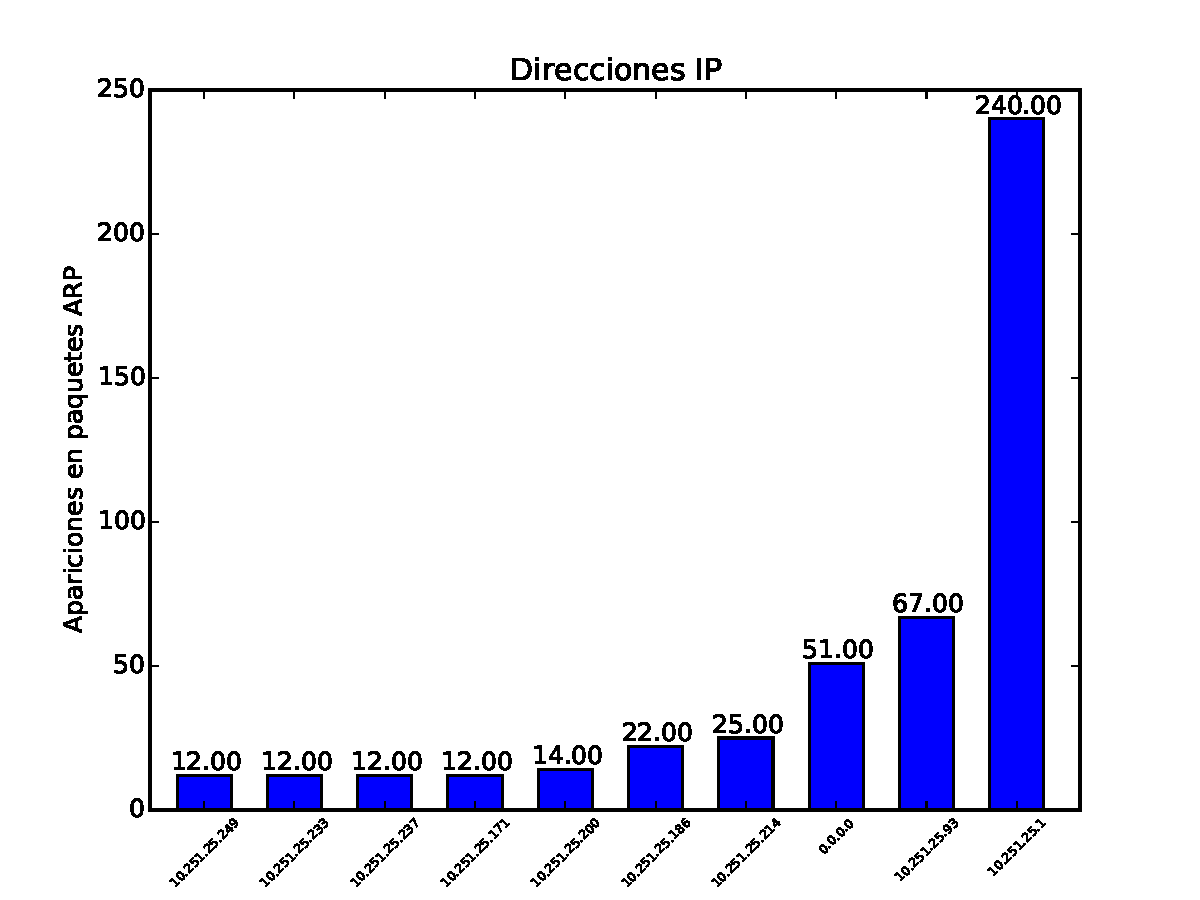
\includegraphics[width=0.8\columnwidth]{graficos/plaza_top_s2.pdf}
%\caption{Red Plaza Oeste}
%\end{center}
%\end{figure}

\begin{table}[H]
\centering
\caption{Red Plaza Oeste}
\label{my-label}
\begin{tabular}{@{}llll@{}}
\toprule
Direccion IP  & Apariciones & Informacion & Apariciones / Total \\ \midrule
10.251.25.214 & 25          & 3.171       & 0.076               \\
10.251.25.93  & 36          & 2.806       & 0.109               \\
0.0.0.0       & 51          & 2.458       & 0.155               \\
10.251.25.1   & 209         & 1.047       & 0.635              
\end{tabular}
\end{table}

%\begin{figure}[H]
%\begin{center}
%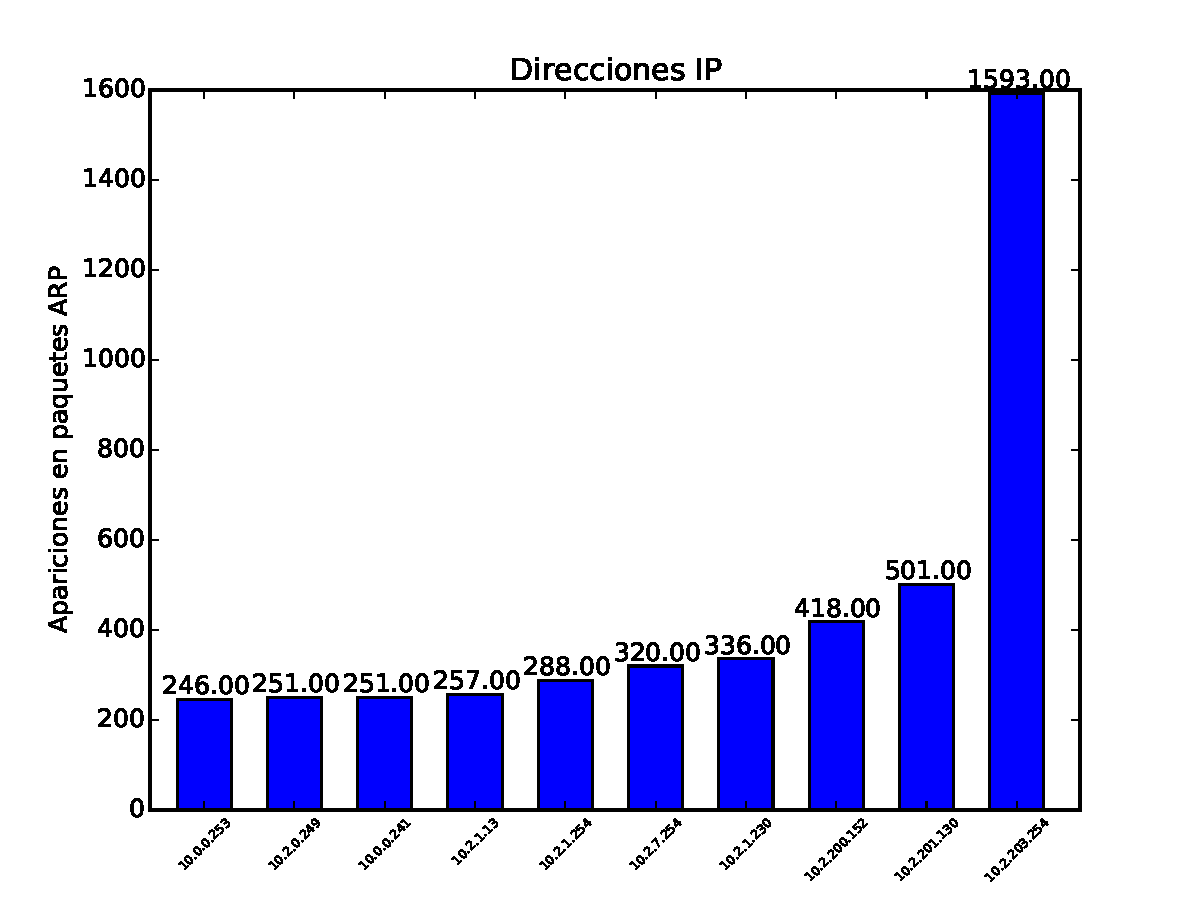
\includegraphics[width=0.8\columnwidth]{graficos/dc_top_s2.pdf}
%\caption{Red Laboratorios DC}
%\end{center}
%\end{figure}

\begin{table}[H]
\centering
\caption{Red Laboratorios DC}
\label{my-label}
\begin{tabular}{@{}llll@{}}
\toprule
Direccion IP & Apariciones & Informacion        & Apariciones / Total 5566 \\ \midrule
10.2.7.249   & 123         & 4.500              & 0.022                    \\
10.2.5.254   & 131         & 4.437              & 0.023                    \\
10.2.6.254   & 150         & 4.302              & 0.026                    \\
10.2.7.23    & 156         & 4.263              & 0.028                    \\
0.0.0.0      & 158         & 4.250              & 0.029                    \\
10.2.3.254   & 163         & 4.219              & 0.030                    \\
10.2.7.13    & 175         & 4.148              & 0.031                    \\
10.2.7.250   & 182         & 4.109              & 0.032                    \\
10.2.203.125 & 200         & 4.014              & 0.035                    \\
10.2.7.4     & 206         & 3.985              & 0.037                    \\
10.2.0.187   & 226         & 3.892              & 0.040                    \\
10.2.200.231 & 235         & 3.853              & 0.042                    \\
10.0.0.253   & 246         & 3.807              & 0.044                    \\
10.2.0.249   & 251         & 3.787              & 0.045                    \\
10.0.0.241   & 251         & 3.787              & 0.045                    \\
10.2.1.13    & 257         & 3.764              & 0.046                    \\
10.2.1.254   & 288         & 3.650              & 0.051                    \\
10.2.7.254   & 320         & 3.544              & 0.057                    \\
10.2.1.230   & 336         & 3.495              & 0.060                    \\
10.2.200.152 & 418         & 3.277              & 0.075                    \\
10.2.201.130 & 501         & 3.096              & 0.090                    \\
10.2.203.254 & 1568        & 1.955              & 0.281                    \\ \bottomrule
\end{tabular}
\end{table}

Una de las suposiciones que teníamos, era que por el funcionamiento de la red Wi-Fi, la gran mayoría de los paquetes irían dirigidos hacia un nodo principal, el cual después se encargaría de redirigirlos al destino apropiado. Como podemos ver, esto ocurrió en ambos casos, hay un nodo el cual tiene muchas mas apariciones que el resto.

A pesar de que los resultados satisfacían nuestras expectativas, nos sorprendió que el margen de diferencia entre el nodo principal y el resto no sea mayor, con lo cual los otros nodos también están enviando paquetes ARP a nodos que no son el principal, esto sera estudiado mas adelante.
%\begin{figure}[H]
%\begin{center}
%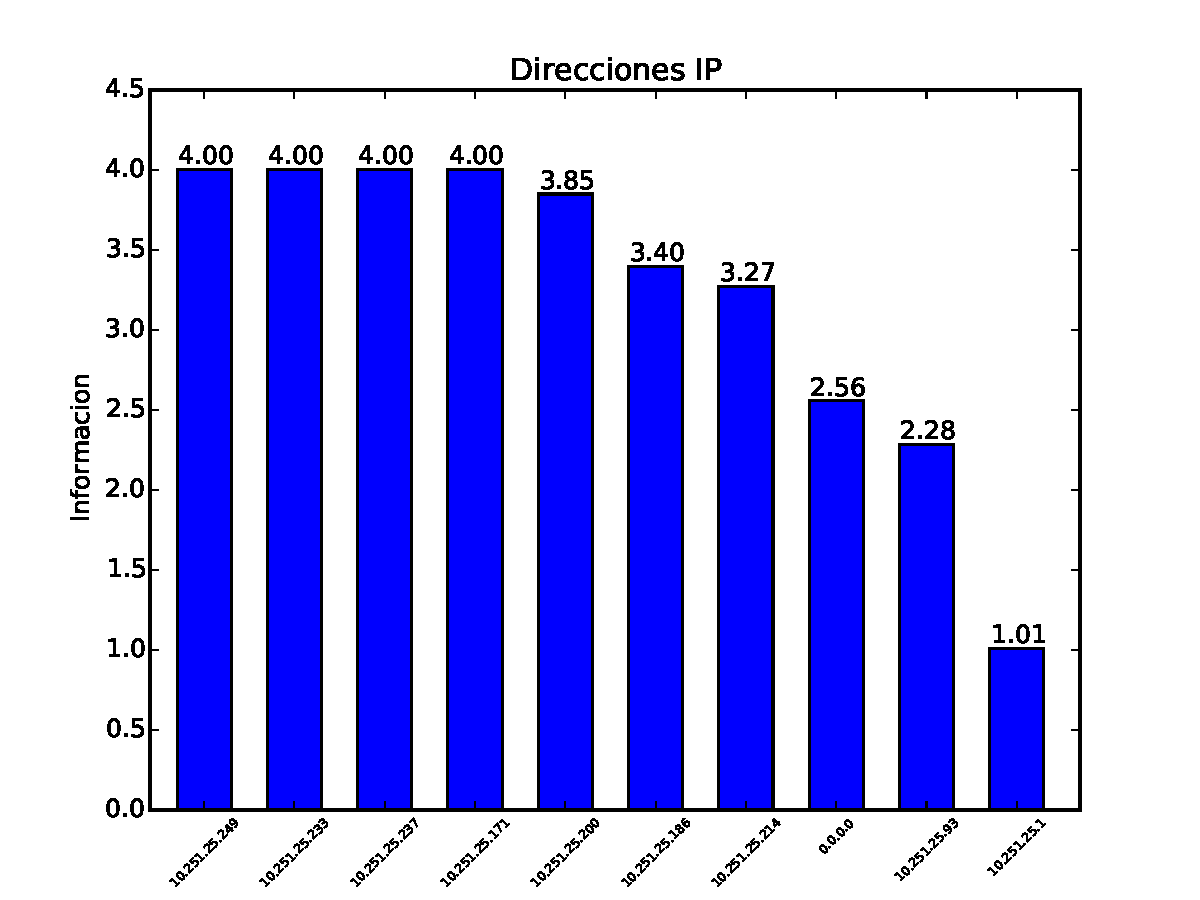
\includegraphics[width=0.8\columnwidth]{graficos/plaza_top_inf_s2.pdf}
%\caption{Red Plaza Oeste}
%\end{center}
%\end{figure}
%
%\begin{figure}[H]
%\begin{center}
%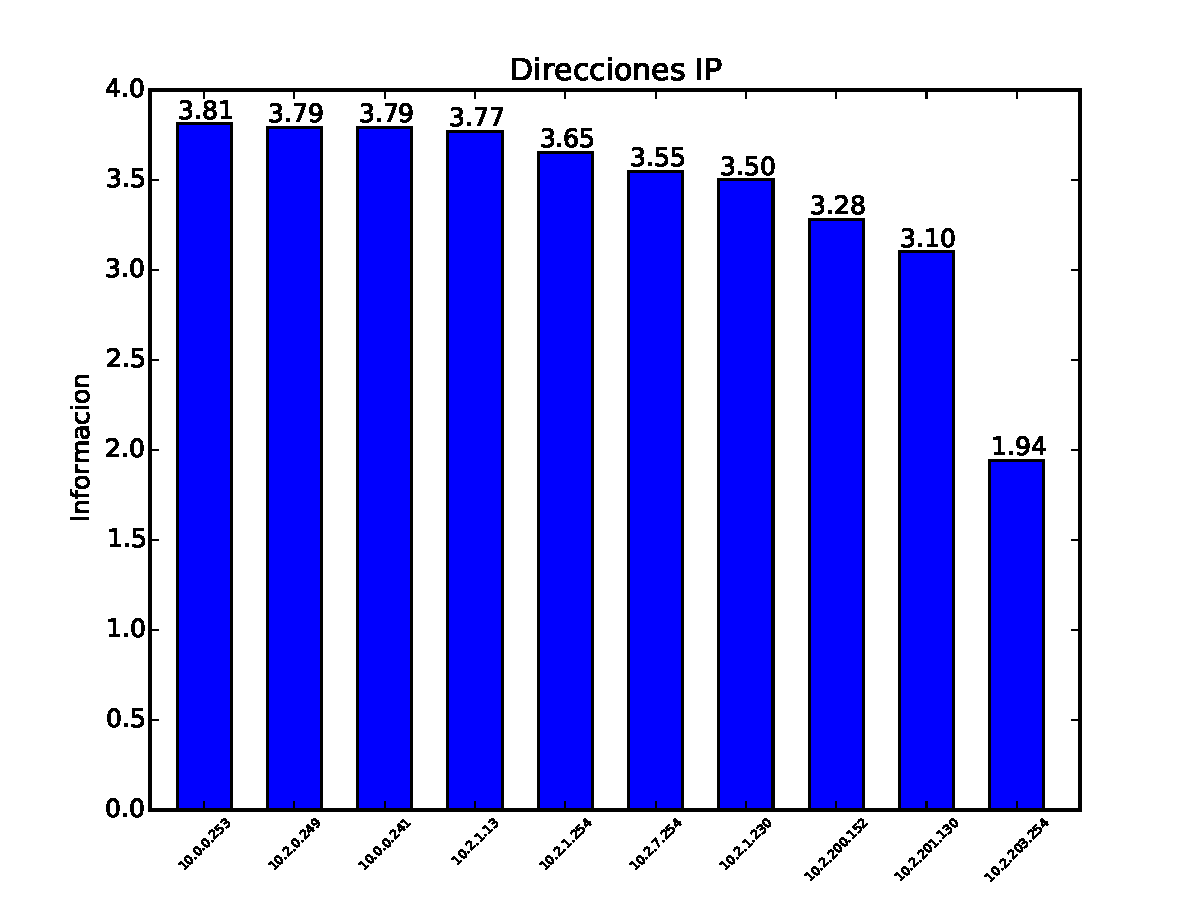
\includegraphics[width=0.8\columnwidth]{graficos/dc_top_inf_s2.pdf}
%\caption{Red Laboratorios DC}
%\end{center}
%\end{figure}

La entropia para estas dos redes fue:

\begin{table}[H]
\centering
\caption{Entropia}
\label{my-label}
\begin{tabular}{ll}
\hline
Red         & Entropia \\ \hline
Plaza Oeste & 3.1724   \\
Laboratorios DC    & 4.6459   \\ \hline
\end{tabular}
\end{table}

Una cosa interesante a destacar, es que la entropia es mucho mayor tomando como símbolos las direcciones IP que los tipos de protocolos, esto ocurre en ambas redes. Esto creemos que se debe principalmente a las siguientes razones:

\begin{itemize}
	\item La cantidad de protocolos es considerablemente menor que la cantidad de direcciones IP posibles, en la practica unicamente vimos tres protocolos en uso
	\item En las redes Wi-Fi, vimos que los nodos que suelen enviar paquetes de tipo \textit{who-has} son aquellos que quieren conectarse a la red, estos suelen tener direcciones IP diferentes a las que ya se encuentran en el sistema, con lo que tenemos que agregar un nuevo símbolo
	\item Es posible que el tamaño de la muestra no haya sido suficiente, y que se necesiten mas tiempo de \textit{sniffeo} para poder calcular bien la entropia
\end{itemize}

Este ultimo punto es particularmente interesante para nosotros, ya que es posible que la muestra tomada no sea significativa del trafico de la red y no sea suficiente para estimar las probabilidades, efectivamente afectando la entropia de la red. También seria interesar estudiar si las políticas de asignación de IP de la red y el uso de la misma terminan amortizando el segundo punto, ya que si el sistema reasigna direcciones siempre que puede, mientras mas grande sea la muestra la diferencia entre el nodo principal y el resto potencialmente seria mayor. Para probar esta teoría, planteamos un experimento simple que consiste en tomar parte de la captura (la mitad de la muestra original), y contrastar los resultados de dicha parte con los totales, con esto podemos estimar si el tiempo puede afectar considerablemente la entropia de la red. Los resultados fueron:

%\begin{figure}[H]
%\begin{center}
%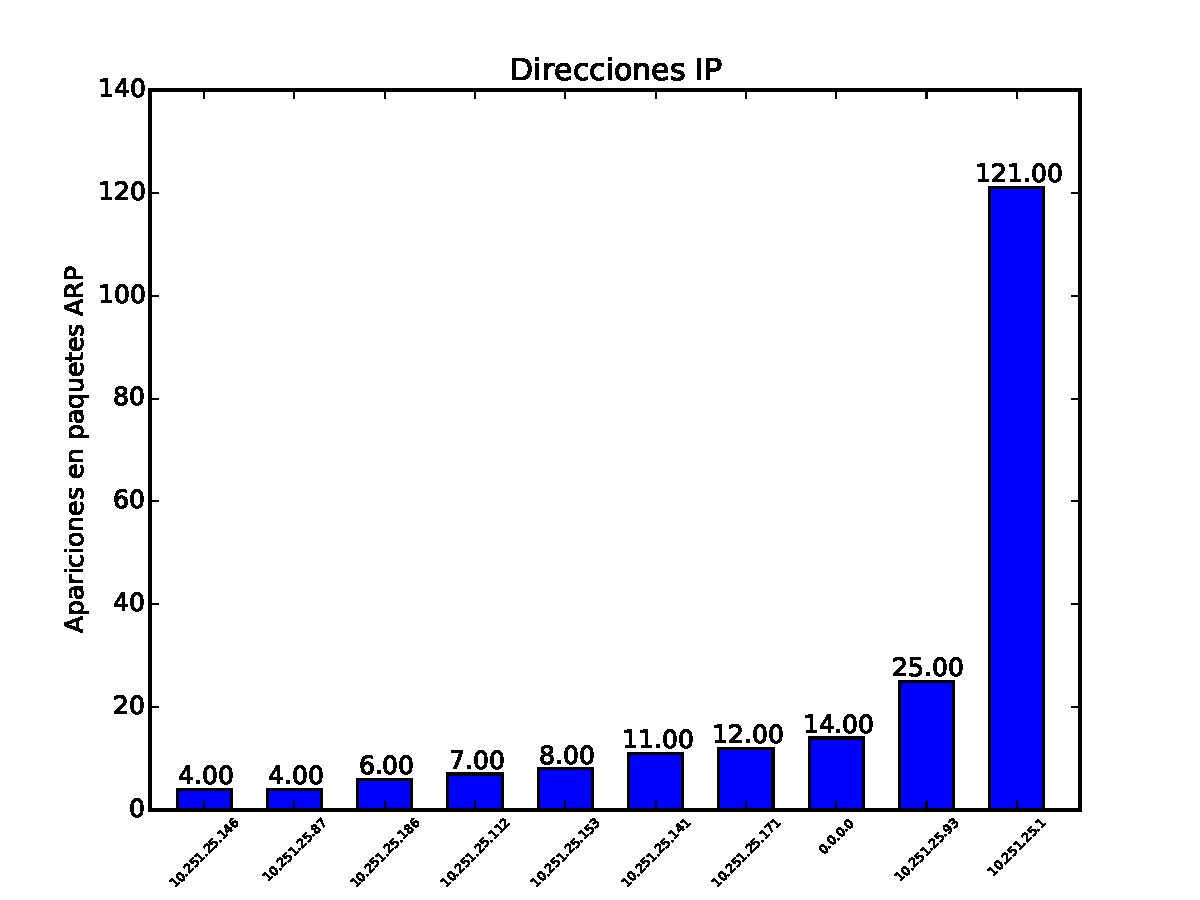
\includegraphics[width=0.8\columnwidth]{graficos/plaza_parcial_s2.pdf}
%\caption{Red Plaza Oeste}
%\end{center}
%\end{figure}

\begin{table}[H]
\centering
\caption{Red Plaza Oeste}
\label{my-label}
\begin{tabular}{@{}llll@{}}
\toprule
Direccion IP & Apariciones & Informacion & Apariciones / Total \\ \midrule
10.251.25.93 & 25          & 2.451       & 0.151               \\
10.251.25.1  & 121         & 0.874       & 0.733               \\ \bottomrule
\end{tabular}
\end{table}

%\begin{figure}[H]
%\begin{center}
%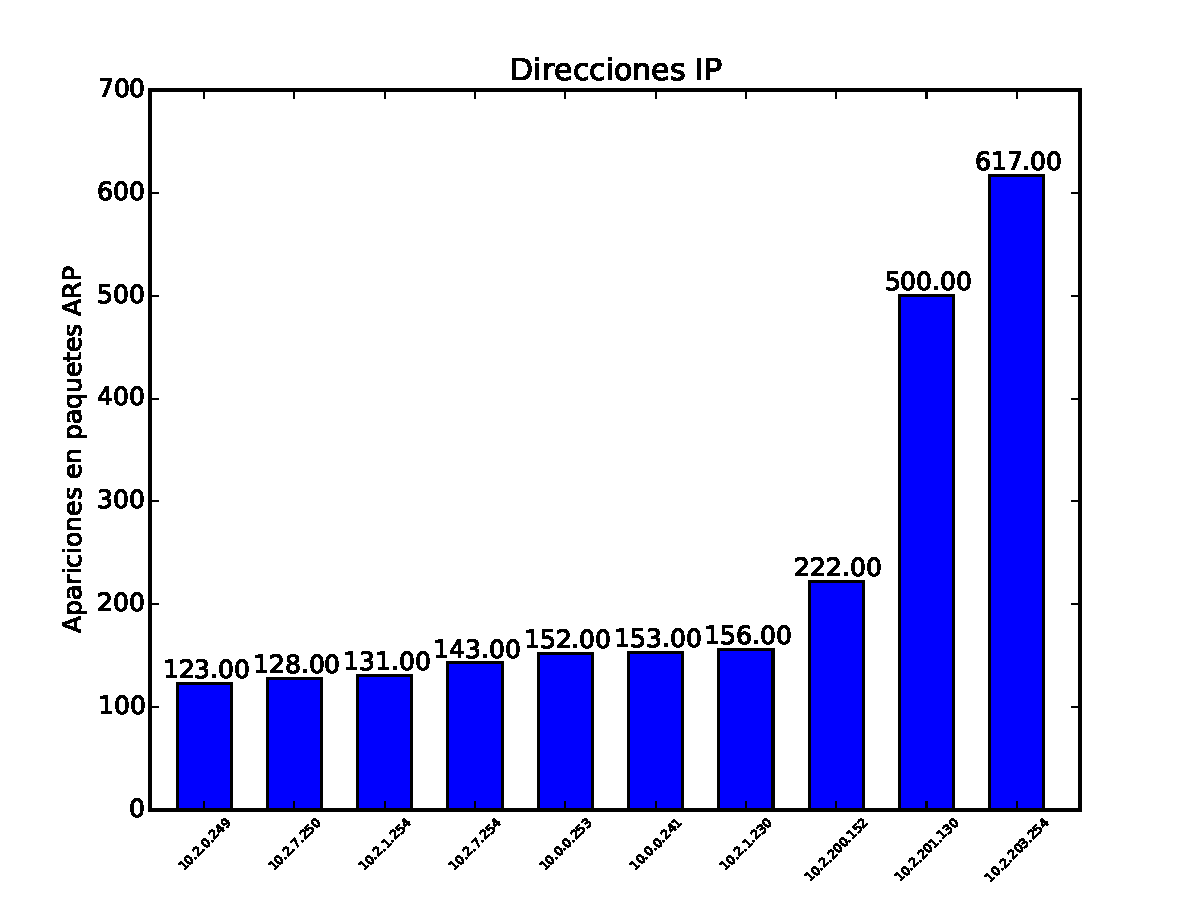
\includegraphics[width=0.8\columnwidth]{graficos/dc_parcial_s2.pdf}
%\caption{Red Laboratorios DC}
%\end{center}
%\end{figure}

\begin{table}[H]
\centering
\caption{Red Laboratorios DC}
\label{my-label}
\begin{tabular}{@{}llll@{}}
\toprule
Direccion IP & Apariciones & Informacion        & Apariciones / Total \\ \midrule
10.2.7.249   & 66          & 4.432   & 0.023               \\
10.2.3.254   & 68          & 4.402  & 0.024               \\
10.2.200.119 & 80          & 4.240  & 0.028               \\
10.2.201.165 & 83          & 4.203  & 0.029               \\
0.0.0.0      & 96          & 4.057  & 0.034               \\
10.2.203.125 & 100         & 4.017  & 0.030               \\
10.2.7.4     & 103         & 3.987  & 0.035               \\
10.2.7.23    & 106         & 3.958 & 0.038               \\
10.2.0.187   & 106         & 3.958 & 0.038               \\
10.2.7.13    & 107         & 3.949 & 0.038               \\
10.2.1.13    & 121         & 3.826  & 0.043               \\
10.2.0.249   & 123         & 3.810 & 0.044               \\
10.2.7.250   & 128         & 3.770 & 0.045               \\
10.2.1.254   & 131         & 3.747 & 0.047               \\
10.2.7.254   & 143         & 3.659 & 0.051               \\
10.0.0.253   & 152         & 3.598 & 0.054               \\
10.0.0.241   & 153         & 3.591  & 0.054               \\
10.2.1.230   & 156         & 3.572  & 0.056               \\
10.2.200.152 & 222         & 3.219 & 0.079               \\
10.2.201.130 & 500         & 2.407  & 0.179               \\
10.2.203.254 & 617         & 2.197 & 0.221               \\ \bottomrule
\end{tabular}
\end{table}

%\begin{figure}[H]
%\begin{center}
%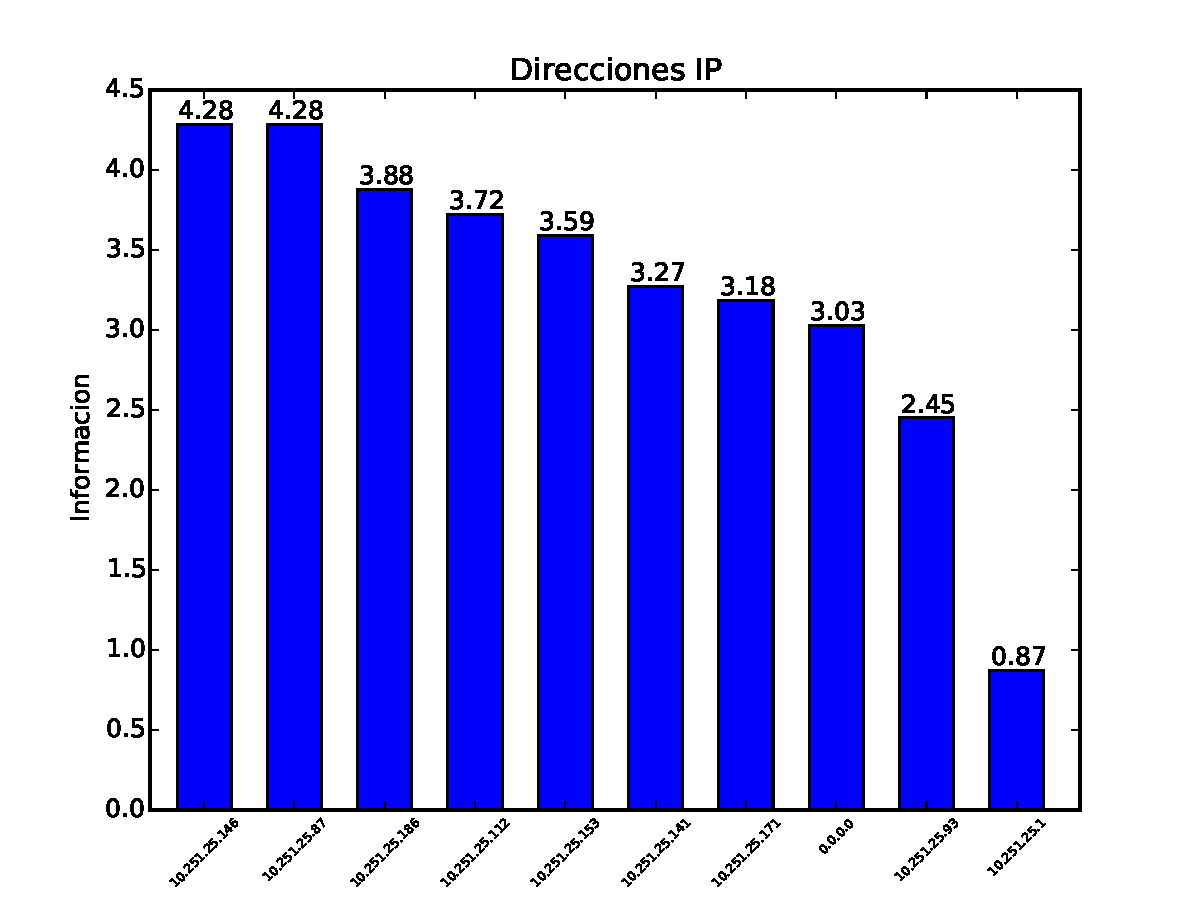
\includegraphics[width=0.8\columnwidth]{graficos/plaza_parcial_inf_s2.pdf}
%\caption{Red Plaza Oeste}
%\end{center}
%\end{figure}

%\begin{figure}[H]
%\begin{center}
%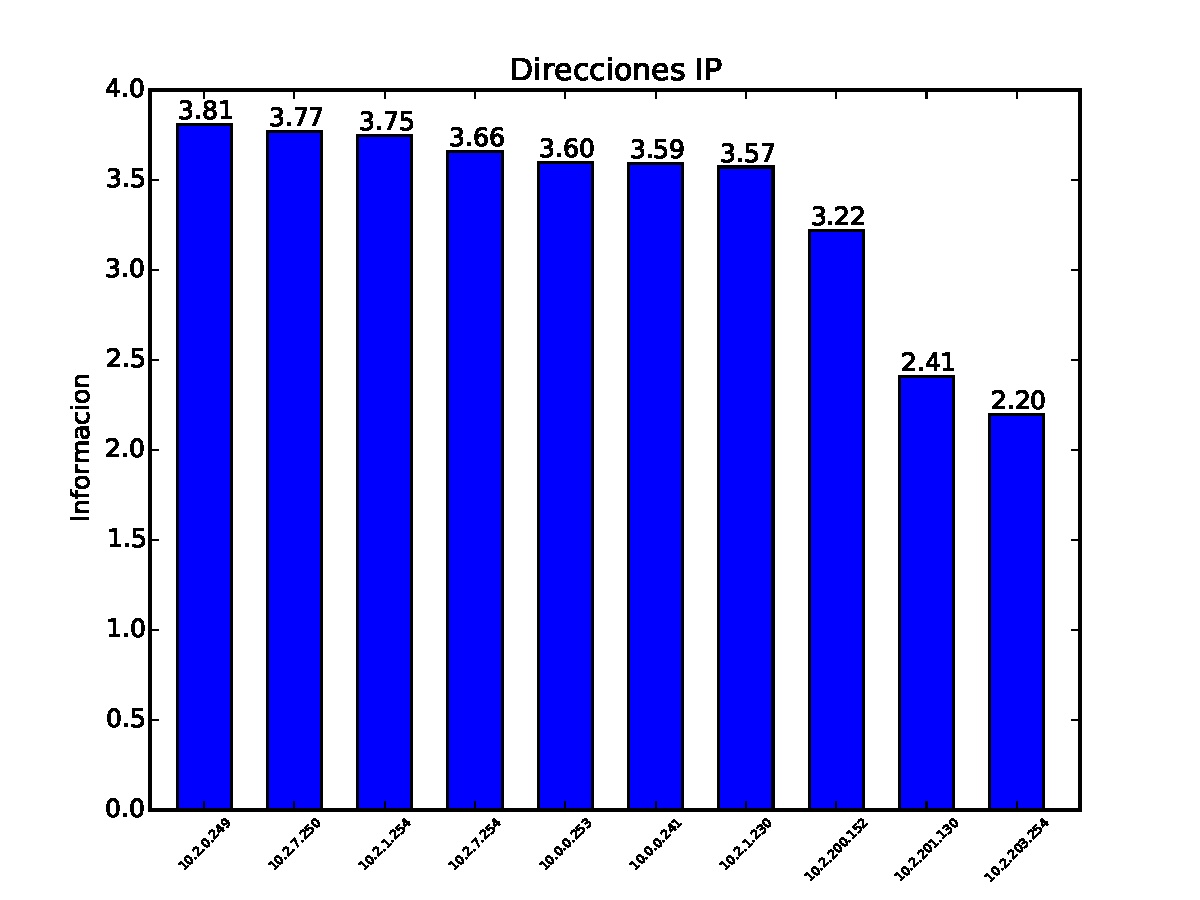
\includegraphics[width=0.8\columnwidth]{graficos/dc_parcial_inf_s2.pdf}
%\caption{Red Laboratorios DC}
%\end{center}
%\end{figure}

La entropia para estas dos redes fue:

\begin{table}[H]
\centering
\caption{Entropia}
\label{my-label}
\begin{tabular}{ll}
\hline
Red         & Entropia \\ \hline
Plaza Oeste & 2.8027   \\
Laboratorios DC    & 4.5887   \\ \hline
\end{tabular}
\end{table}

Como podemos ver, si bien hubo diferencia entre los resultados parciales y los finales, esta diferencia no fue muy grande, esto lo podemos interpretar de dos formas. Por un lado, podríamos pensar que la captura tiene que ser mucho mas grande (del orden de días) para que las políticas de asignación de IP tengan efecto sobre la entropia, o podemos pensar que dichas políticas no van a tener peso significativo sobre los resultados finales. Particularmente nos inclinamos por la segundo opción, ya que hay muchos elementos en juego a la hora de tomar una medición, particularmente el canal puede estar mas o menos congestionado, afectando la medición, esto podemos verlo contrastando la muestra reducida de Laboratorios DC con la muestra completa, allí en la completa se ve claramente marcada la dirección \texttt{10.2.203.254} por sobre el resto, tanto en información como en apariciones, mientras que en la muestra parcial no es encuentra tan marcada.

En general, la red respondió de la manera que esperábamos, pudimos identificar un nodo principal el cual aparece en muchas mas ocasiones que el resto en ambas redes. Si bien la diferencia en cantidad de apariciones de dichos nodos respecto al resto no fue tan significativa, cumplen con el criterio de símbolo distinguido planteado anteriormente, con lo cual podemos marcarlos como símbolos distinguidos en sus respectivos canales. Por ultimo queda analizar el caso de la red hogareña y determinar si el símbolo distinguido de la misma corresponde con la dirección del enrutador.

\subsubsection{Red hogareña}

Como era de esperar, los resultados en la red hogareña fueron considerablemente mas reducidos que en las redes publicas, con lo cual optamos por colocar la totalidad de las direcciones en la tabla. Los resultados fueron las siguientes:

%\begin{figure}[H]
%\begin{center}
%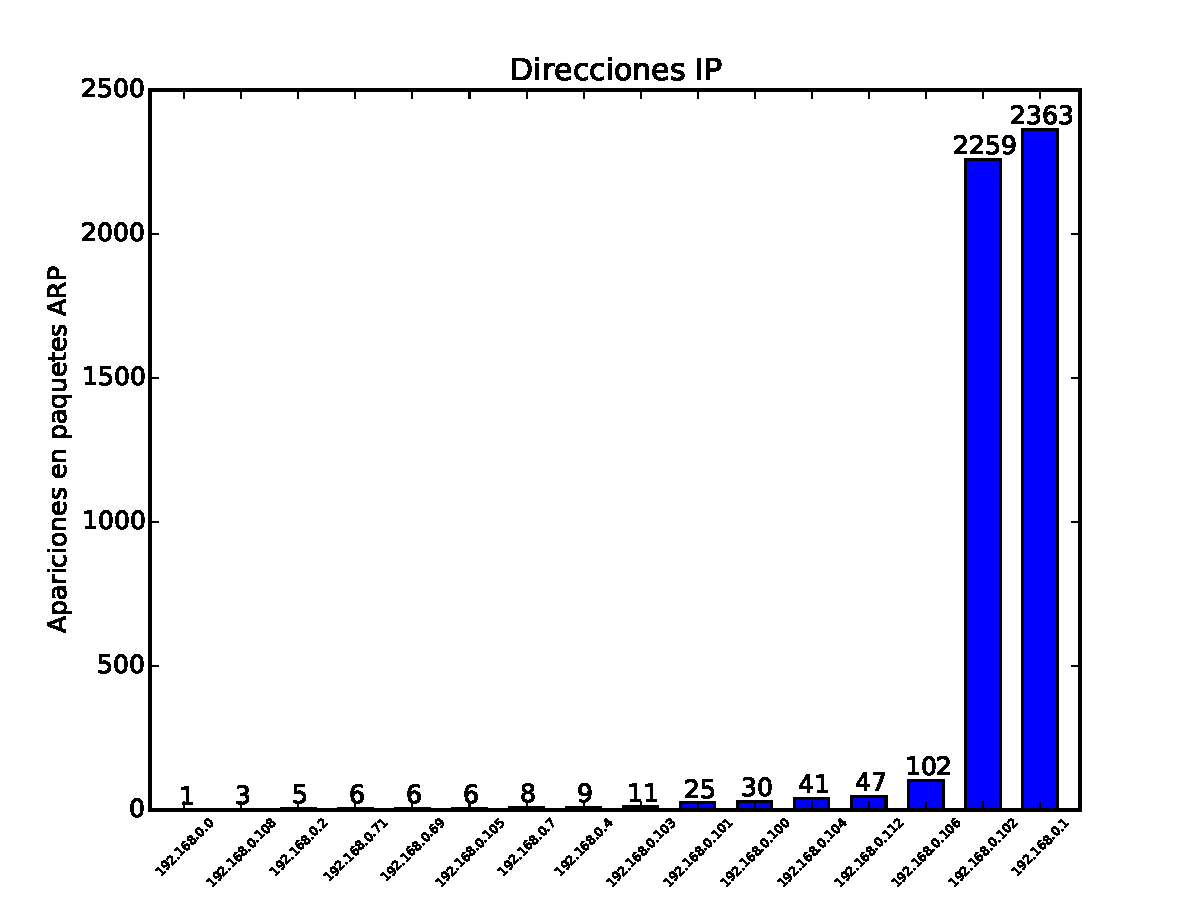
\includegraphics[width=0.8\columnwidth]{graficos/hogar_s2.pdf}
%\caption{Red hogareña}
%\end{center}
%\end{figure}
%
%\begin{figure}[H]
%\begin{center}
%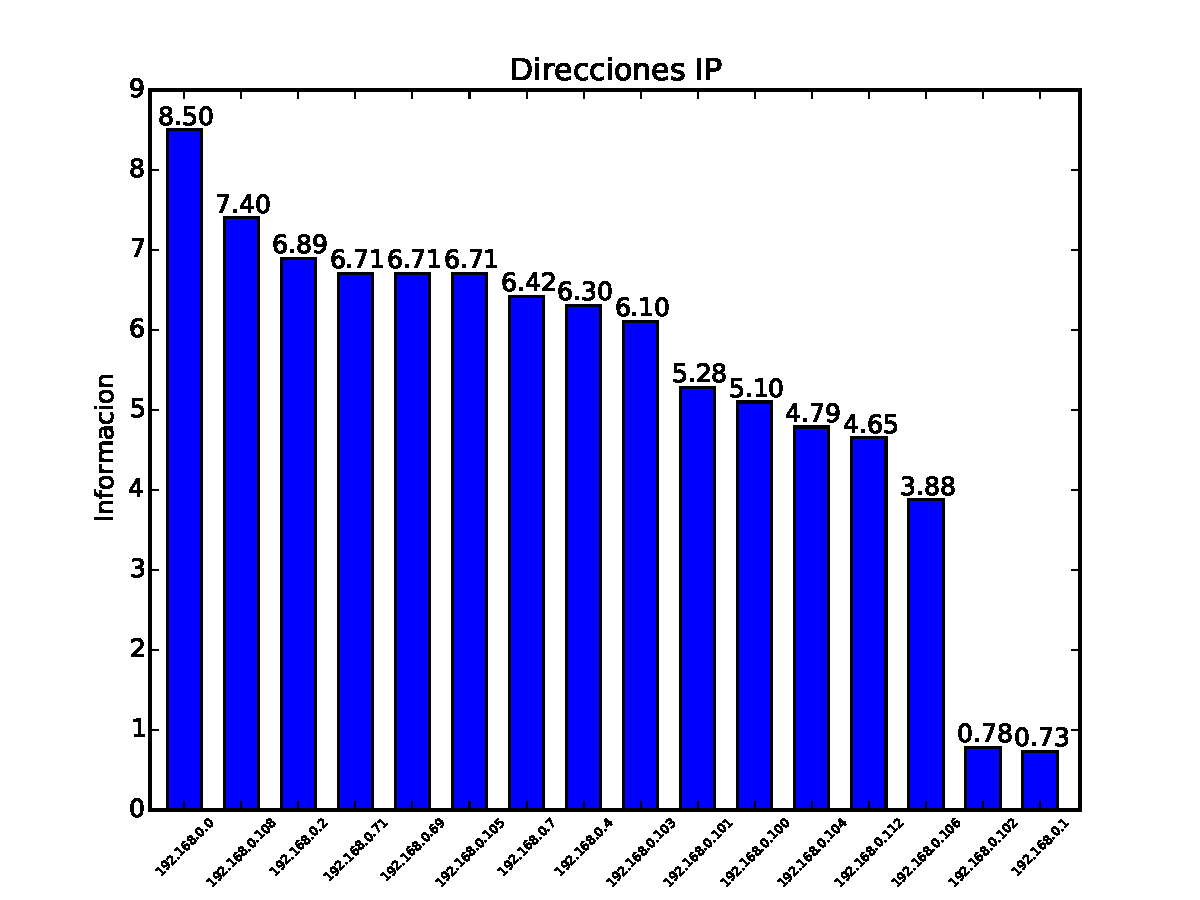
\includegraphics[width=0.8\columnwidth]{graficos/hogar_inf_s2.pdf}
%\caption{Red hogareña}
%\end{center}
%\end{figure}

\begin{table}[H]
\centering
\caption{Red Hogareña}
\label{my-label}
\begin{tabular}{@{}llll@{}}
\toprule
Direccion IP  & Apariciones & Informacion & Apariciones / Total \\ \midrule
192.168.0.0   & 1           & 8.501       & 0.0001              \\
192.168.0.108 & 3           & 7.402       & 0.0001              \\
192.168.0.2   & 5           & 6.892       & 0.001               \\
192.168.0.71  & 6           & 6.709       & 0.001               \\
192.168.0.69  & 6           & 6.709       & 0.001               \\
192.168.0.105 & 6           & 6.709       & 0.001               \\
192.168.0.7   & 8           & 6.422       & 0.001               \\
192.168.0.4   & 9           & 6.304       & 0.001               \\
192.168.0.103 & 11          & 6.103       & 0.002               \\
192.168.0.101 & 25          & 5.282       & 0.005               \\
192.168.0.100 & 30          & 5.100       & 0.006               \\
192.168.0.104 & 41          & 4.787       & 0.008               \\
192.168.0.112 & 47          & 4.651       & 0.009               \\
192.168.0.106 & 102         & 3.876       & 0.020               \\
192.168.0.102 & 2259        & 0.778       & 0.458               \\
192.168.0.1   & 2363        & 0.733       & 0.480               \\ \bottomrule
\end{tabular}
\end{table}

La entropia para esta red fue de 1.0057.

%\begin{table}[H]
%\centering
%\caption{Entropia}
%\label{my-label}
%\begin{tabular}{ll}
%\hline
%Red         & Entropia \\ \hline
%Red hogareña & 1.0057   \\
%\end{tabular}
%\end{table}

Debido a que conocemos como esta formada esta red, sabemos que la dirección IP del enrutador es \texttt{192.168.0.1}. Si bien la dirección IP \texttt{192.168.0.102} también apareció repetidas veces, esto se debe a que la computadora desde donde se tomo la muestra, ya que era uno de los pocos dispositivos conectados a la red activamente utilizando la misma, con lo cual su presencia fue mayor en la medición. Como podemos apreciar, utilizando el criterio expuesto anteriormente, vemos que el símbolo distinguido en la red es efectivamente la dirección IP \texttt{192.168.0.1}, con lo cual podemos dar una verificación básica de nuestra teoría, ya que el símbolo se corresponde con el enrutador.

\subsection{Paquetes de control ARP}

En la sección anterior hablamos de paquetes que no eran enviados hacia el nodo principal, ademas de esto, nos dimos cuenta que varios de ellos tenían una forma bastante particular, tras consultar diferentes recursos nos dimos cuenta que varios de ellos eran paquetes de control. Nos topamos con los siguientes:

\begin{itemize}
	\item Dirección IP \texttt{0.0.0.0}: Estos paquetes se utilizan para revisar si una dirección IP se encuentra en uso por algún host, la idea es que un nodo al recibir una dirección IP para usar, envia este paquete, y si recibe un \textit{is-at} de otro nodo quiere decir que la dirección que pretendía utilizar esta en uso
	\item Misma dirección IP de fuente y destino: Este es un paquete bastante particular, sirve para que los diferentes hosts en la red tengan sus tablas de dirección IP y MAC actualizadas. La idea es que al recibir el paquete y verificar que las direcciones origen y destino son iguales, el host revisa si tiene la dirección MAC en su tabla, en caso de tenerla actualiza la dirección IP almacenada si es que esta cambio por la dirección que figura en el paquete. Mantener las relaciones IP y MAC actualizadas es sumamente importante en la red, ya que eso puede ahorrarnos una cantidad significativa de tiempo a la hora de manejar el trafico.
\end{itemize}

Las apariciones de estos paquetes consideramos que terminaron quitandole bastante peso al nodo central respecto a los demás, haciendo que la entropia sea mayor.

\section{Conclusiones}

Es bastante interesante ver como los diferentes conceptos de teoría de la información aplican en canales reales, particularmente considerando que fueron planteados en 1948 cuando las redes modernas no existian. Desde el punto de vista de las redes Wi-Fi puntualmente, vimos como la comunicación es sumamente centralizada y dominada por IPv4, lo primero se puede ver claramente en los paquetes ARP los cuales en nuestras muestras estan en gran parte dirigidos a un único nodo, mientras que lo segundo no solamente se ve a simple vista, sino que ademas es esperable considerando que la Internet funciona sobre IPv4.

Como estudio a futuro, seria interesante hacer un \textit{sniffeo} durante el lapso de uno o mas días, para poder ver si las proporciones obtenidas con la fuente $S_1$ se mantienen, o si eventualmente el nodo principal se impone respecto al resto aumentando aun mas la diferencia entre estos. También consideramos importante analizar las diferentes técnicas de ARP Spoofing, y analizar cuan factible es realizar dichos ataques y el alcance de los mismos, particularmente hacer spoofing del gateway, en redes Wi-Fi esto es sumamente interesante ya que al ser centralizada podríamos redirigir el trafico y administrar el acceso a la red.
%\subsection{Proporcion de trafico local e Internet}
%
%METER ESTO EN DISTINCION DE NODOS
%
%Nos parecio tambien interesante analizar la proporcion de trafico local respecto al trafico que va hacia Internet, nuestra teoria es que en la red publica del Plaza Oeste todo el trafico se destina a Internet a traves del enrutador. Por otro lado, la red Laboratorios-DC, al ser de la facultad, seguramente tengo mas trafico interno.